\section{Options de g\'en\'erateur}
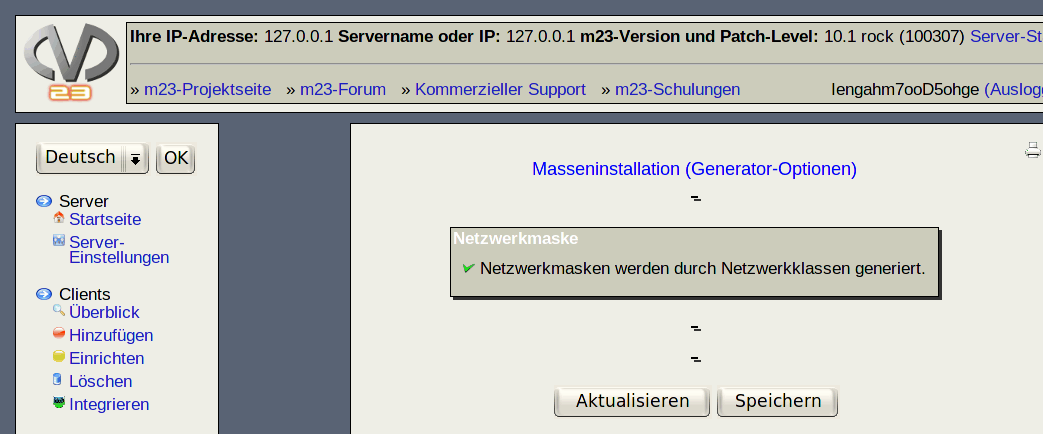
\includegraphics[scale=0.4]{/mdk/doc/manual/screenshots/fr/mi_step3.png} \\
Ici, vous pouvez entrer les param\`etres pour les g\'en\'erateurs des propri\'et\'es suivantes:\\
\begin{itemize}
\item \textbf{Nom de poste client}: Ici, vous pouvez d\'efinir la base des noms des postes client et un num\'ero de commencement. Puis, le nombre de noms des postes client n\'ecessaire sera cr\'e\'e selon le sch\'ema $\langle$base du nom du poste client$\rangle$ $\langle$num\'ero d'ordre$\rangle$. Des noms de postes client qui existent d\'ej\`a seront saut\'es pendant ce processus. Exemple: base des noms des postes client=m23client, num\'ero de commencement=12 g\'en\`ere les noms de postes client m23client12, m23client13, ...\\
\item \textbf{Nom d'entr�e dans le syst�me}: C'est le nom avec lequel l'utilisateur peut entrer dans le syst\`eme du poste client. Vous avez le choix entre deux m\'ethodes de sa g\'en\'eration. La m\'ethode de l'accroissement arbitraire se comporte comme la g\'en\'eration chez \textit{$\ll$Nom de poste client$\gg$}. En plus, vous pouvez choisir un mot de passe construit de la premi\`ere lettre du pr\'enom et du surnom compl\`et. (\textit{$\ll$G�n�rer � partir du pr�nom et du nom de famille$\gg$}).\\
\item \textbf{Pr�nom}: La g\'en\'eration des pr\'enoms (qui sont les nom de l'entr\'ee dans le syst\`eme au m\^eme temps) sera ex\'ecut\'e de la m\^eme fa\c{c}on.\\
\item \textbf{Adresse IP}: Ici, vous pouvez d\'eterminer les limites d'adresses IP, dans lesquelles des adresses IP libres doivent \^etre cherch\'ees. Il seront seulement g\'en\'er\'es des adresses IP qui ne sont pas d\'ej\`a utilis\'ees par des postes client m23. Pourtant, vous pouvez d\'ecider que toute adresse IP doit \^etre contact\'ee avant l'usage. Si un ou plusieurs ordinateurs r\'epondent, leurs adresses IP ne seront pas utilis\'ees.\\
\item \textbf{Masque r�seau}: Les masques de r\'eseau seront calcul\'ees automatiquement d'apr\`es le sch\'ema des classes de r\'eseau.\\
Ceci est par d\'efinition:\\
\begin{tabular}{|c|c|c|}
\hline
\`a partir de & jusqu'\`a & Masque de r\'eseau\\
	 \hline
0.0.0.0 & 127.255.255.255 & 255.0.0.0\\
	 \hline
128.000.000.000 & 191.255.255.255 & 255.255.0.0\\
	 \hline
192.000.000.000 & 255.255.255.255 & 255.255.255.0\\
	 \hline
\end{tabular}
\item \textbf{Premi�re entr�e dans le syst�me}: Pour cette entr\'ee dans le syst\`eme, les mots de passe peuvent \^etre g\'en\'er\'es compl\`etement au hasard (\textit{$\ll$Mots de passe cr�es au hasard$\gg$}) ou par un sch\'ema de hasard qui est plus simplement m\'emorable pour les hommes (\textit{$\ll$Mots de passe cr�es avec PwGen$\gg$}). Le longueur des mots de passe g\'en\'er\'es peut \^etre vari\'e entre 6 et 8 caract\`eres. Il est recommand\'e de garder le longeur programm\'e de 8 caract\`eres.\\
\item \textbf{ID de l'utilisateur}: Ici, vous devez d\'efinir le num\'ero de commencement \`a partir duquel des identit\'es d'utilisateur libres doivent \^etre cherch\'ees et utilis\'ees.\\
\item \textbf{ID du groupe}: Ici, d\'efinez le num\'ero de commencement, \`a parir duquel des identit\'es de groupe libres doivent \^etre cherch\'ees et utilis\'ees.\\
\end{itemize}
